\documentclass{article}

% packages
\usepackage{hyperref}
\usepackage{graphicx}
\usepackage[american]{circuitikz}
\usepackage{siunitx}
\usepackage{amsmath}

\begin{document}
	\subsubsection{Resistance, Reactance, Impedance and Admittance}
	\href{https://tech-notes.quantmasters.in/concept-of-impedance-admittance-2/}{Useful website link.} \\\\
	\begin{center}
		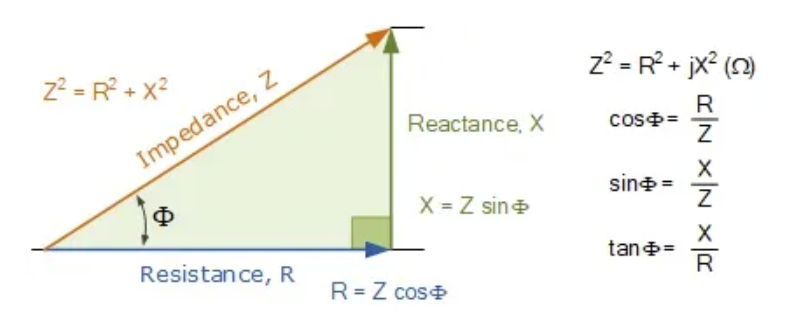
\includegraphics[width=0.5\textwidth]{imgs/impedancetriangle.png} \\
	\end{center}
	Impedance : Ability to stop/resist current at a specific frequency. \\
	Resistance : Ability to stop electric current flow. \\
	Reactance : Ability to store and release energy. \\
	Admittance : Ability to allow/let current flow through at a specific frequency. \\
	\begin{itemize}
		\item if energy is stored and release in \textbf{magnetic field}, reactance is inductive. $+jX_L$, voltage leads current by 90 (voltage peak first as time progress)
		\item if energy is stored and released in \textbf{eletric field}, reactance is capacitive. $-jX_C$, current leads voltage by 90 (current peak first as time progress)
	\end{itemize}
	
	\ \\So given this circuit\\\\
	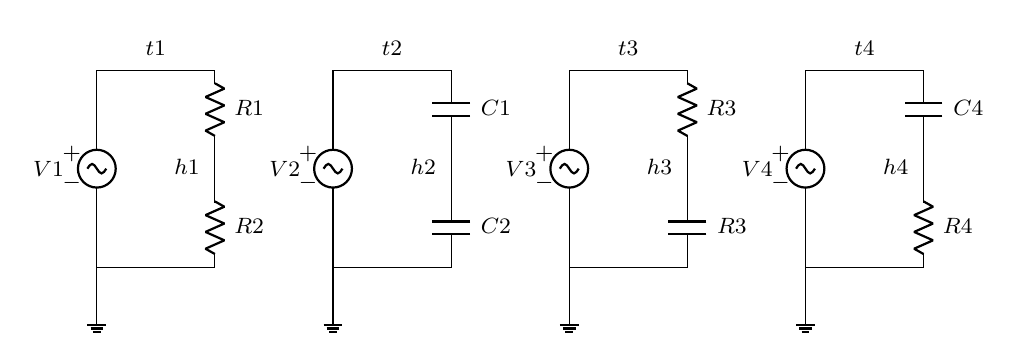
\begin{tikzpicture}[scale=0.5, font=\footnotesize]
		\ctikzset{bipoles/length=0.8cm}
		\draw (0,0) node[ground]{} -- ++(0,3) to[sV<=$V1$] ++(0,1) -- ++(0,2) to[short=$t1$] ++(3, 0) to[R=$R1$] ++(0,-2) to[short, l_=$h1$] ++(0,-1) to[R=$R2$] ++(0,-2) -- ++(-3,0);
		\draw (6,0) node[ground]{} -- ++(0,3) to[sV<=$V2$] ++(0,1) -- ++(0,2) to[short=$t2$] ++(3, 0) to[C=$C1$] ++(0,-2) to[short, l_=$h2$] ++(0,-1) to[C=$C2$] ++(0,-2) -- ++(-3,0);
		\draw (12,0) node[ground]{} -- ++(0,3) to[sV<=$V3$] ++(0,1) -- ++(0,2) to[short=$t3$] ++(3, 0) to[R=$R3$] ++(0,-2) to[short, l_=$h3$] ++(0,-1) to[C=$R3$] ++(0,-2) -- ++(-3,0);
		\draw (18,0) node[ground]{} -- ++(0,3) to[sV<=$V4$] ++(0,1) -- ++(0,2) to[short=$t4$] ++(3, 0) to[C=$C4$] ++(0,-2) to[short, l_=$h4$] ++(0,-1) to[R=$R4$] ++(0,-2) -- ++(-3,0);
	\end{tikzpicture}
	\begin{center}
		\[f = 1\times10^6 = 1\ \si{\mega\hertz}, \ All\ Vx = \sin(2\pi ft)\]
		\[All\ Cx = 1\ \si{\micro\farad},\ All\ Rx = \frac{1}{2\pi fC} = 0.159154\ \si{\ohm}\]
	\end{center}
	\textbf{For circuit with $V1$}
	\[I(R1) = \frac{1\ \si{\volt}}{2\times0.159154\si{\ohm}}\ =\ 3.1416\ \si{\ampere}\]
	Current is a sine wave with peak amplitude of $3.1416\ \si{\ampere}$, and it is in phase with the voltage sinusoidal source. Just like a voltage divider.\\\\
	\begin{center}
		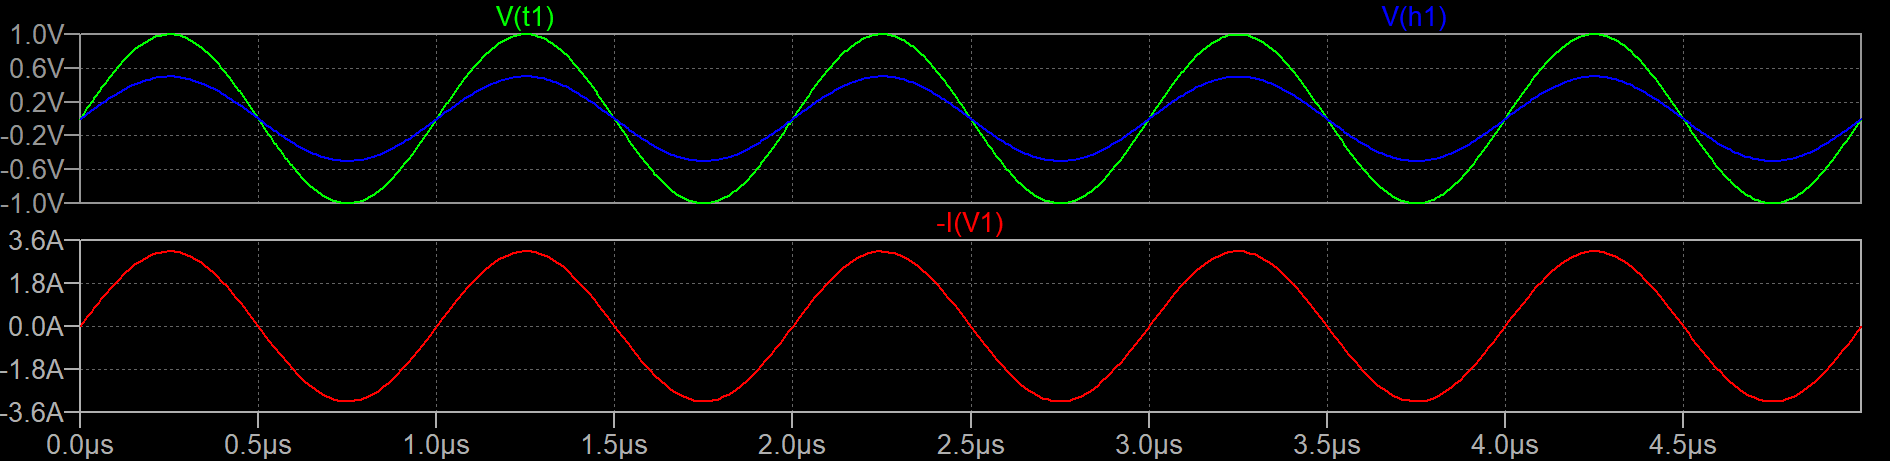
\includegraphics[width=\textwidth]{imgs/v1_circuit.png} \\
	\end{center}
	\textbf{For circuit with $V2$} \\
	Amplitude wise(at node $h2$) it is also like a voltage divider, the signal at node $h2$ is half of $t2$, that's obvious.
	\[V(h2)=V(t2)\times \frac{Z_{C1}}{Z_{C1}+Z_{C2}}=V(t2)\times \frac{-j\frac{1}{2\pi fC_{1}}}{-j\frac{1}{2\pi fC_{1}}+-j\frac{1}{2\pi fC_{2}}}=\frac{V(t2)}{2}\]
	Current wise it is 90 degree out of phase, current lead voltage by $\frac{\pi}{2}$
	\[I(C1)=\frac{V(t2)}{-j\frac{2}{2\pi fC_{1}}}=\frac{V(t2)}{-j\frac{2}{2\pi fC_{1}}}\times\frac{+j\frac{2}{2\pi fC_{1}}}{+j\frac{2}{2\pi fC_{1}}}=0+j\frac{V(t2)\times \frac{2}{2\pi fC_{1}}}{(\frac{2}{2\pi fC_{1}})^2}\]
	\[\arctan(\frac{\frac{V(t2)\times \frac{2}{2\pi fC_{1}}}{(\frac{2}{2\pi fC_{1}})^2}}{0})=\arctan(\infty)=90\si{\degree}\]
	This is saying that our current signal will start at positive 90 degrees which is peak amplitude.
	\begin{center}
		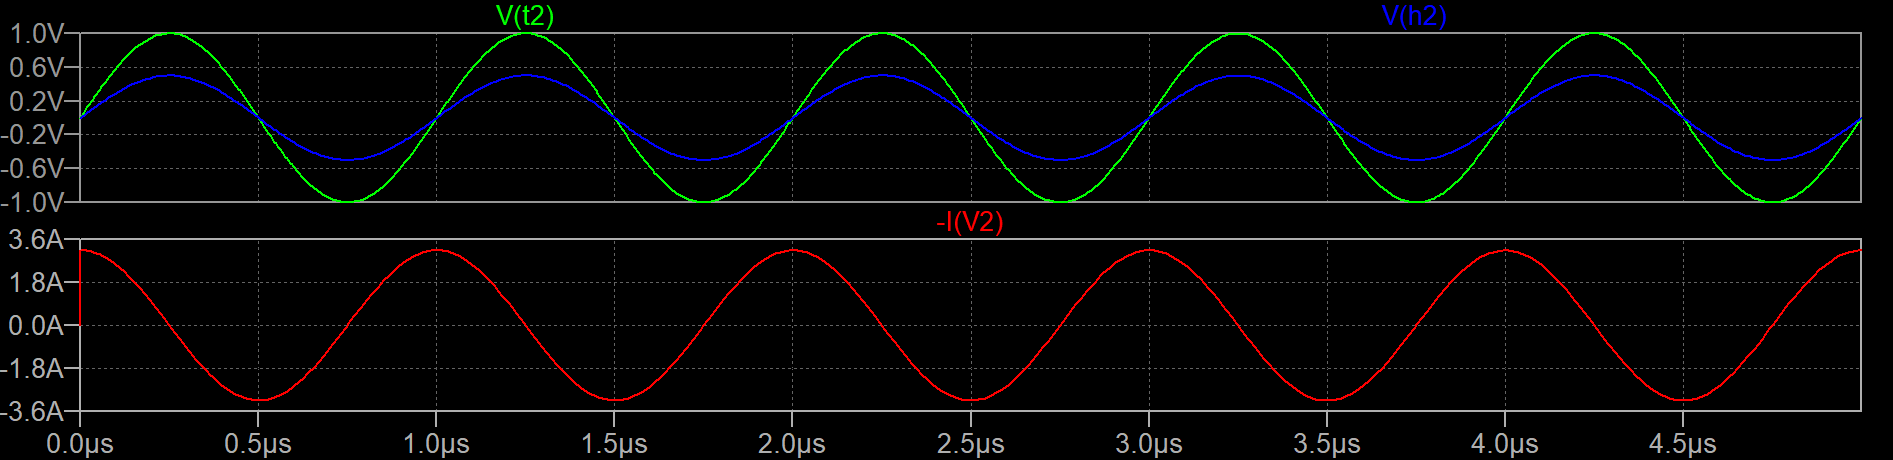
\includegraphics[width=\textwidth]{imgs/v2_circuit.png} \\
	\end{center}
	\textbf{For circuit with $V3$} \\
	At node $h3$, it is also like a voltage divider but noticed it is not divided by half.
	\begin{align*}
		V(h3)=V(t3)\ \frac{Z_{C3}}{Z_{R3}+Z_{C3}}=V(t3)\ \frac{-j0.159154}{0.159154-j0.159154}=V(t3)\ \frac{-j}{1-j} \\
		=V(t3)\ \frac{1-j}{2}
	\end{align*}
	\begin{align*}
		\Big\|V(t3)\ \frac{1-j}{2}\Big\|&=V(t3)\ \sqrt{\left(\frac{1}{2}\right)^2+\left(\frac{1}{2}\right)^2}=0.707108\ V(t3) \\
		\angle V(t3)\ \frac{1-j}{2}&=arctan\left(\frac{-\frac{1}{2}}{\frac{1}{2}}\right)=-45\si{\degree}
	\end{align*}
	-45 \si{\degree} means it's "lagging" original sine wave by 45 degrees, moving the original waveform to the right. \\
	Note that we're taking the voltage across the capacitor $C3$. $V(t3)-V(h3)$ is the voltage across the resistor, and its phase is +45 \si{\degree}.
	\begin{gather*}
		I(C3)=\frac{V(t3)}{0.159154-j0.159154}=\frac{V(t3)}{0.318308}(1+j) \\
		\Big\|\frac{V(t3)}{0.318308}(1+j)\Big\|=4.4429\ V(t3)\\
		\angle\frac{V(t3)}{0.318308}(1+j)=+45\si{\degree}
	\end{gather*}
	Current wise it is leading voltage $V(h3)$ by 45 \si{\degree}, notice that it is not our original 90 \si{\degree}. We can intuitively explain this as the resistance is slowing down the current, which makes charging and discharging the capacitor slower, thus we have a phase compromise between having both resistor and having both capacitors. 
	\begin{center}
		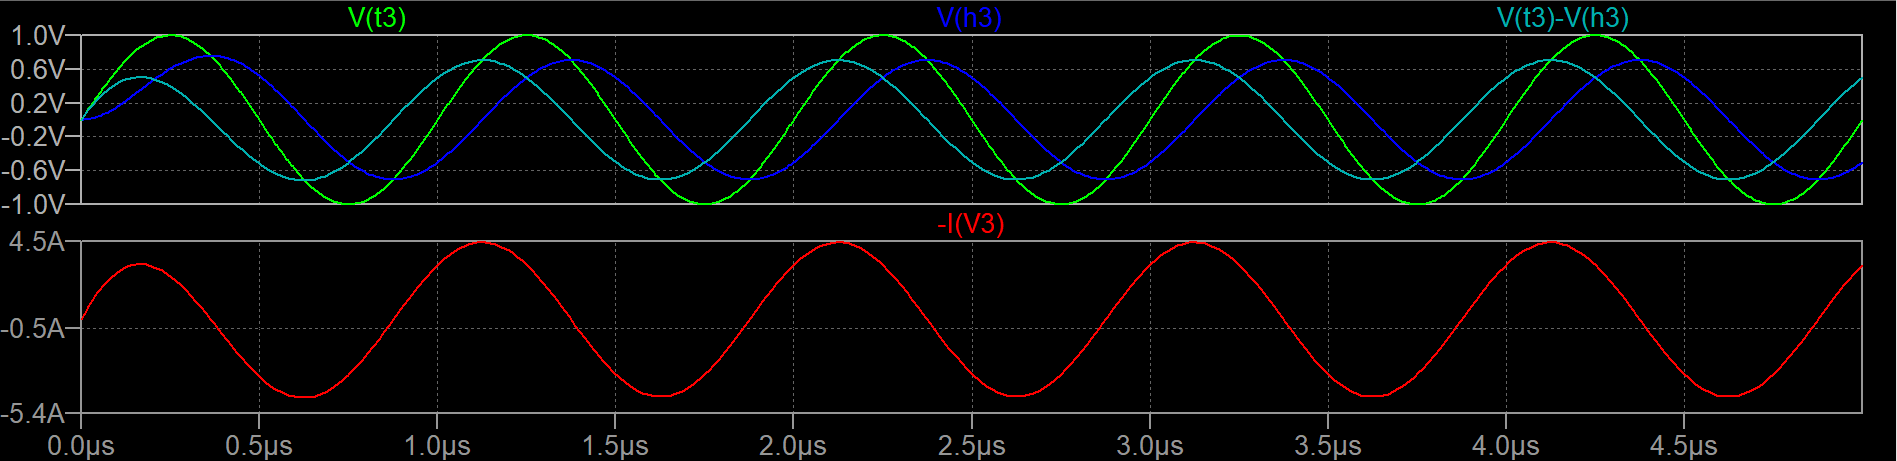
\includegraphics[width=\textwidth]{imgs/v3_circuit.png} \\
	\end{center}
		
\end{document}